%
% main.tex -- Paper zum Thema arctan
%
% (c) 2020 Hochschule Rapperswil
%
\chapter{Interpolation und numerische Ableitung\label{chapter:interdiff}}
\lhead{Interpolation und numerische Ableitung}
\rhead{}
\begin{refsection}
\chapterauthor{Andreas Müller}
\index{Interpolation}%
\index{Ableitung, numerische}%
\index{numerische Ableitung}%
\index{Muller, Andreas@Müller, Andreas}%

{\parindent0pt
In} Kapitel~\ref{chapter:interpolation} wurde gezeigt, wie man durch
Interpolation gute Approximationen einer Funktion in einem Interval
finden kann.
Für äquidistante Stützstellen ist das Interpolationspolynom vor allem in
der Mitte des Intervalls sehr genau.
Man kann daher versuchen, diese Approximation durch das Interpolationspolynom
auch für eine Approximation der Ableitung der Funktion zu verwenden, indem
man das Interpolationspolynom ableitet.
\index{Interpolationspolynom}%
Am Ende dieses Prozesses sollte sich eine Formel ergeben, welche die
Ableitung näherungsweise aus Funktionswerten in der Nähe des
interessierenden Punktes bestimmt, ganz ähnlich wie das aus der
Taylor-Reihe abgeleitete, in Kapitel~\ref{chapter:ableitung} beschriebene
Verfahren.
\index{Taylor-Reihe}%
Dieses Kapitel führt die Berechnung der Gewichte der Funktionswerte durch
und untersucht mit Hilfe der Fourier-Transformation, was man von dem Verfahren
erwarten kann.
\index{Fourier-Transformation}%

%
% problem.tex
%
% (c) 2020 Prof Dr Andreas Müller, Hochschule Rapperswil
%
\section{Problemstellung
\label{section:pde:problem}}
\rhead{Problemstellung}
Gewöhnliche Differentialgleichungen werden durch eine einzige Funktion
$f\colon \mathbb R\times\mathbb R^n: (t,x)\mapsto f(t,x)$ beschrieben,
werden.
Eine Lösung der Differentialgleichung
\begin{equation}
\frac{dx}{dt} = f(t,x)
\label{pde:eqn:ode}
\end{equation}
mit der Anfangsbedingung
\[
x(t_0) = x_0
\]
ist eine Funktion $x(t)$ mit $x(t_0)=x_0$ derart, dass 
\[
\frac{dx(t)}{dt} = f(t, x(t)).
\]
Das Definitionsgebiet der Lösungsfunktion $x(t)$ ist ein Intervall
der Form $[t_0,a]$ mit $a>t_0$.

Für eine partielle Differentialgleichung ist die Situation wesentlich
komplizierter.
Zunächst gibt es Ableitungen der gesuchten Funktion $u(x_1,\dots,x_n)$
nach allen unabhängigen Variablen zu
berücksichtigen, so dass eine explizite Form der Differentialgleichung
wie in~\eqref{pde:eqn:ode} grundsätzlich nicht mehr möglich ist.
Das Definitionsgebiet ist eine fast beliebige Teilmenge
$\Omega\subset\mathbb R^n$ eines $n$-dimensionalen Raumes.
Insbesondere kann das Definitionsgebiet sehr viel komplizierter sein
als im Falle einer gewöhnlichen Differentialgleichungen.
Die Form des Gebietes hat einen wesentlichen Einfluss auf die Lösungen
der Differentialgleichung.
Schliesslich wird es nicht mehr genügen, Werte in nur einem Randpunkt
des Gebietes zu kennen, wie das bei einer gewöhnlichen Differentialgleichung
der Fall war.
Vielmehr ist es eine nichttriviale Frage, auf welchem Teil des Randes
$\partial\Omega$ von $\Omega$ welche Funktions- oder Ableitungswerte
vorgegeben werden müssen, damit die Lösung der Differentialgleichung
eindeutig bestimmt ist.

Der Einfachheit halber betrachten wir in diesem Kapitel nur partielle
Differentialgleichungen für eine skalare Funktion $u=u(x_1,\dots,x_n)$.
In diesem Abschnitt geht es darum zu klären, wie genau ein solches
Problem gestellt werden muss.
In Abschnitt~\ref{subsection:pde:gebiet} studieren wir ein sinnvolles
Definitionsgebiet für die Differentialgleichung.
In Abschnitt~\ref{subsection:pde:klassifikation} klassifizieren wir
mögliche Differentialgleichungen bevor wir in
Abschnitt~\ref{subsection:pde:randbedingungen} Randbedingungen und
in Abschnitt~\ref{subsection:pde:loesungen} Lösungen beschreiben.

\subsection{Gebiet und Rand
\label{subsection:pde:gebiet}}
Eine partielle Differentialgleichung sucht eine Funktion
\[
u\colon \Omega\to\mathbb R
\]
$u(x_1,\dots,x_n)$, für die Beziehungen zwischen den partiellen
Ableitungen nach den unabhängigen Variablen gelten.
Für alle Punkte einer Menge $\Omega\subset\mathbb R^n$ muss
als eine Gleichung ähnlich wie zum Beispiel
\[
\Delta u
=
\frac{\partial^2 u}{\partial x_1^2}
+
\dots
+
\frac{\partial^2 u}{\partial x_n^2}
=
0
\qquad
\forall \;
(x_1,\dots,x_n)\in \Omega
\]
gelten, $\Delta$ ist der {\em Laplace-Operator}.
\index{Laplace-Operator}
Diese Beobachtung schränkt die Art der Menge $\Omega$ bereits ein,
wie im Folgenden diskutiert werden soll.

\begin{figure}
\centering
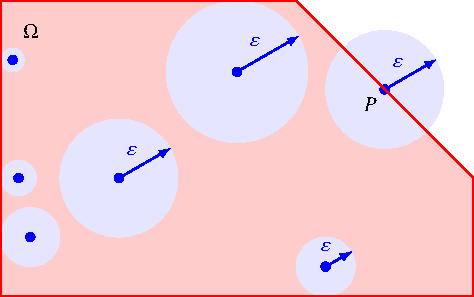
\includegraphics{chapters/70-pde/images/offen.pdf}
\caption{Jeder innere Punkt einer Menge hat eine $\varepsilon$-Umgebung, 
die ebenfalls in der Menge enthalten ist.
Jede Umgebung des Punktes $P$ enthält aber auch Punkte ausserhalb der
Menge $\Omega$, $P$ ist daher ein Randpunkt.
\label{buch:pde:figure:offen}}
\end{figure}

Die Ableitung einer Funktion $u(x_1,\dots,x_n)$ in einem Punkt
$x_0=(x_{0,1},\dots,x_{0,n})$ ist eine lineare Funktion 
$Du(x_{0,1},\dots,x_{0,n}) $ derart, dass
\[
u(x_1,\dots,x_n) - u(x_{0,1},\dots,u_{0,n})
=
Du(x_{0,1},\dots,x_{0,n})\cdot (x-x_0) + o(|x-x_0|).
\]
Das Symbol $o(|x-x_0|)$ beschreibt eine Funktion, die schneller als
ihr Argument gegen $0$ geht, so dass für den Grenzwert des
Quotienten 
\[
\lim_{x\to x_0}\frac{o(|x-x_0|)}{|x-x_0|} = 0
\]
gilt.
Der Grenzwert bedeutet, dass es für jedes $\varepsilon>0$ eine Umgebung
$U_\delta(x_0)=\{x\;|\; |x-x_0|<\delta\}$ gibt derart, dass
\[
\bigl|
u(x)-u(x_0) - Du(x_0)\cdot (x-x_0)
\bigr|
< \varepsilon\cdot |x-x_0|
\qquad\forall x\in U_\delta(x_0)
\]
ist.
Dies ist nur sinnvoll, wenn die ganze Umgebung $U_{\delta}(x_0)\subset \Omega$
im Definitionsgebiet $\Omega$ der Differentialgleichung vorhanden ist.
Dies führt auf die folgende Definition (siehe auch Abbildung~\ref{buch:pde:figure:offen}.

\begin{definition}
Eine Menge $\Omega$ heisst {\em offen}, wenn mit jedem Punkt $x\in \Omega$
auch eine offene Umgebung $U_{\delta}(x)\subset\Omega$ darin enthalten ist.
Ein {\em Gebiet} ist eine offene Menge in $\mathbb R^n$.
\end{definition}

Gebiete sind also genau die sinnvollen Definitionsgebiete für eine partielle
Differentialgleichung.
Es reicht allerdings nicht, dass die Funktion $u$ auf $\Omega$ definiert
ist, da ja auch noch Randwerte erfüllt werden müssen.

\begin{figure}
\centering
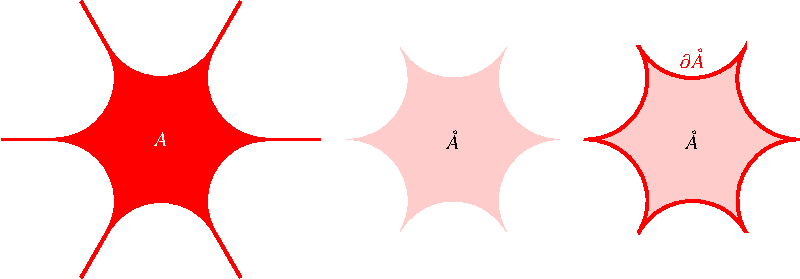
\includegraphics{chapters/70-pde/images/gebiet.pdf}
\caption{Inneres und Rand einer Punktmenge $A$ in der Ebene.
Die sechs Strahlen der Menge $A$ links können nichts zu den Randwerten
einer partiellen Differentialgleichunb beitragen, weil sie keinen
Einfluss auf Werte in inneren Punkten (Mitte) haben können.
Randwerte müssen daher nur auf einem Teil des Randes $\partial\mathring{A}$
des Inneren (rechts) spezifiziert werden.
\label{buch:pde:figure:gebiet}}
\end{figure}

\begin{definition}
Der {\em Abschluss} $\bar{\Omega}$ einer Menge $\Omega\subset\mathbb R^n$ ist
die Menge aller Punkte in $\mathbb R^n$, die Grenzwerte von Folgen in
$\Omega$ sind.
Das {\em Innere} $\mathring{A}$ einer Menge $A$ ist die Menge aller Punkte
$x$ derart, dass es eine Umgebung $U_\delta(x)$ gibt, die ganz in $A$
enthalten ist: $U_{\delta}(x)\subset A$.
\end{definition}

Alternativ kann man den Abschluss auch charakterisieren als die Menge
aller Punkte $x\in\mathbb R^n$, für die jede beliebige Umgebung
$U_\delta(x)$ auch Punkte von $\Omega$ enthält, also
$U_\delta(x)\cap \Omega\ne \emptyset$.
Ein Gebiet ist offen, daher ist $\mathring\Omega=\Omega$.

Die Lösung einer partiellen Differentialgleichung wird im Allgemeinen erst
festgelegt sein, wenn zusätzlich Werte auf Teilen des ``Randes'' des
Gebietes festgelegt worden sind.
Nur Punkte, die als Grenzwerte von Punkten in $\Omega$ erreicht werden
können, können zu diesem Zweck hinzugezogen werden.

\begin{definition}
Der {\em Rand} $\partial A$ einer Menge $A\subset\mathbb R^n$ ist
$\partial A=\bar{A}\setminus\mathring{A}$.
\end{definition}

Während also eine Differentialgleichung typischerweise auf einem
Gebiet $\Omega$ definiert ist, muss die gesuchte Lösungsfunktion
sogar auf auf dem Abschluss $\bar{\Omega}$ definiert sein.
Die Lösung wird im Allgemeinen erst dadurch festgelegt, dass zusätzlich
Werte oder Ableitungen auf Teilen des Randes $\partial\Omega$ 
vorgegeben werden.

\subsection{Klassifikation der partiellen Differentialgleichungen
\label{subsection:pde:klassifikation}}
Eine partielle Differentialgleichung beschreibt eine Beziehung 
zwischen den partiellen Ableitungen der Funktion $u(x_1,\dots,x_n)$.
Dies ist auf sehr vielfältige Arten möglich, in die dieser Abschnitt
etwas Ordnung bringen soll.

\subsubsection{Ordnung}
Wie bei den gewöhnlichen Differentialgleichungen klassifizieren wir
auch partielle Differentialgleichungen nach der Ordnung.

\begin{definition}
Die {\em Ordnung} einer partiellen Differentialgleichung ist die
Ordnung der höchsten Ableitung, die in der Differentialgleichung
vorkommt.
\end{definition}

Für die folgende Diskussion reicht es, partielle Differentialgleichungen
zweiter Ordnung zu betrachten.
Die meisten in den Anwendungen vorkommenden Differentialgleichungen
sind von dieser Art, so dass dies eine unwesentliche Einschränkung ist.
Die Erweiterungen für höhere Ordnung sind offensichtlich.

\subsubsection{Linearität}
Die Beziehung zwischen den Ableitungen kann beschrieben werden durch
eine Funktion
\[
F(x_1,\dots,x_n,u,p_1,\dots,p_n,t_{11},t_{12},\dots,t_{nn})
\]
derart, dass nach der Substitution
\begin{align*}
u&\to u(x_1,\dots,x_n)
\\
p_i&\to \frac{\partial u}{\partial x_i}
\\
t_{ij} &Ò\to \frac{\partial^2 u}{\partial x_i\,\partial x_j}
\end{align*}
die Differentialgleichung
\[
F\biggl(
x_1,\dots,x_n,u(x_1,\dots,x_n),
\frac{\partial u}{\partial x_1},\dots,\frac{\partial u}{\partial x_n},
\frac{\partial^2u}{\partial x_1^2},
\frac{\partial^2u}{\partial x_1\,\partial x_2},\dots,
\frac{\partial^2u}{\partial x_n^2}
\biggr)
=0
\]
entsteht.
Für höhere Ordnung werden weitere Variablen benötigt, die für die
höheren Ableitungen stehen.
Die Funktion $F$ kann also dazu verwendet werden, die verschiedenen
möglichen partiellen Differentialgleichungen zu klassifizieren.

Eine partielle Differentialgleichung heisst {\em linear}, wenn die
Funktion $F$ linear ist in den Argumenten $u$, $p_i$ und $t_{ij}$,
wenn also gilt
\begin{align}
F(\dots,\lambda u' + \mu u'',\dots)
&=
\lambda F(\dots,u',\dots) + \mu F(\dots,u'',\dots)
\label{pde:eqn:linearu}
\\
F(\dots,\lambda p'_i+\mu p''_i,\dots)
&=
\lambda F(\dots,p'_i,\dots) + \mu F(\dots,p''_i,\dots)
&&\forall i
\label{pde:eqn:linearp}
\\
F(\dots,\lambda t'_{ij}+\mu t''_{ij},\dots)
&=
\lambda F(\dots,t'_{ij},\dots) + \mu F(\dots,t''_{ij},\dots)
&&\forall i,j.
\label{pde:eqn:lineart}
\end{align}
Eine partielle Differentialgleichung heisst {\em quasilinear}, 
wenn die Funktion $F$ linear ist in den Argumenten $p_i$ und $t_{ij}$,
wenn also die Bedingungen~\eqref{pde:eqn:linearp} und \eqref{pde:eqn:lineart}
gelten.
Linearität in $u$, also die Bedingung~\eqref{pde:eqn:linearu} ist
für eine quaslinieare partielle Differentialgleichung nicht verlangt.

\begin{beispiel}
Die Differentialgleichung
\[
\frac{\partial^2 u}{\partial x_1^2}
+
\frac{\partial^2 u}{\partial x_2^2}
=
0
\]
zweiter Ordnung wird beschrieben durch die Funktion
\[
F(x_1,x_2,u,p_1,p_2,t_{11},t_{12},t_{22})
=
t_{11} + t_{22}.
\]
Diese Funktion ist linear in $t_{11}$ und $t_{22}$.
\end{beispiel}

\begin{beispiel}
Die partielle Differentialgleichung erster Ordnung von Burgers
(Siehe auch Kapitel~\ref{chapter:burgers})
\begin{equation}
\frac{\partial u}{\partial x_1}
+
u
\frac{\partial u}{\partial x_2}
=
0
\label{buch:eqn:burgers}
\end{equation}
wird beschrieben durch die Funktion
\[
F(x_1,x_2,u,p_1,p_2)
=
p_1+up_2.
\]
Diese Funktion ist nicht linear in $u$ und $p_2$, aber linear in
$p_1$ und $p_2$.
\eqref{buch:eqn:burgers} ist also eine quasilineare partielle
Differentialgleichung.
\end{beispiel}

\subsubsection{Lineare Differentialgleichungen zweiter Ordnung}
Ein für die Anwendungen besonders wichtiger Fall sind lineare
Differentialgleichungen zweiter Ordnung.
Für eine solche Gleichung ist die Funktion $F$ immer von der Form
\[
F(x_i,u,p_i,t_{ij})
=
\sum_{i,j=1}^n a_{ij}(x_1,\dots,x_n)t_{ij} + \sum_{i=1}^n b_i(x_1,\dots,x_n) p_i + c(x_1,\dots,x_n) u 
\]
Die Koeffizienten $a_{ij}$, $b_i$ und $c$ dürfen also von den Variablen
$x_1,\dots,x_n$ abhängen, nicht aber von $u$ oder den Ableitungen.
Die Differentialgleichung hat also die Form
\begin{equation}
\sum_{i,j=1}^n
a_{ij}\frac{\partial^2 u}{\partial x_i\,\partial x_j}
+
\sum_{i=1}^n
b_i\frac{\partial u}{\partial x_i}
+
cu
=
f
\label{pde:eqn:eqn2nd}
\end{equation}
Da es in den zweiten Ableitungen nicht auf die Reihenfolge ankommt,
kann die Matrix $a_{ij}$ immer symmetrisch gewählt werden.
Die Matrix $A=(a_{ij})$ heisst die {\em Symbolmatrix} der Differentialgleichung.
\index{Symbolmatrix}

Es stellt sich heraus, dass die Terme zweiter Ordnung, also die 
Matrix $A$, das Verhalten der Lösung wesentlich beeinflussen.
Eine symmetrische Matrix kann durch eine Drehung immer in eine
Diagonalmatrix transformiert werden.
Durch Wechsel des Koordinatensystems kann man also erreichen, dass
\[
A
=
\begin{pmatrix}
\lambda_1&         &      &         \\
         &\lambda_2&      &         \\
         &         &\ddots&         \\
         &         &      &\lambda_n
\end{pmatrix}
\]
ist.
In diesen Koordinaten sind es nur noch die Eigenwerte
$\lambda_1,\dots,\lambda_n$ der Matrix $A$, die das Verhalten der Lösung
bestimmen.

\begin{definition}
Die Differentialgleichung
\eqref{pde:eqn:eqn2nd}
heisst {\em elliptisch}, wenn alle Eigenwerte positiv sind.
Sie heisst {\em hyperbolisch}, wenn alle Eigenwerte bis auf einen negativen
positiv sind.
Sie heisst {\em parabolisch}, wenn alle Eigenwerte bis auf einen
verschwindenden positiv sind.
\end{definition}
\index{elliptische partielle Differentialgleichung}%
\index{hyperbolisch partielle Differentialgleichung}%
\index{parabolisch partielle Differentialgleichung}%

\begin{beispiel}
Die {\em Wellengleichung}
\[
\frac{1}{a^2}\frac{\partial^2 u}{\partial t^2}
=
\Delta u 
\quad\Rightarrow\quad
\Delta u 
-
\frac{1}{a^2}\frac{\partial^2 u}{\partial t^2}
=
0
\]
hat die Symbolmatrix
\[
A=
\begin{pmatrix}
1& &      &              \\
 &1&      &              \\
 & &\ddots&              \\
 & &      &\displaystyle-\frac{1}{a^2}
\end{pmatrix}
\]
$n$ positive und einem negativen Eigenwert, diese Gleichung ist also
hyperbolisch.
Die Lösungen zeigen Wellencharakter und die Werte und ersten
Ableitungen von $u$ zu einem Zeitpunkt $t_0$ bestimmen das Verhalten
der Lösung vollständig.
Eine hyperbolische Differentialgleichung hat also eine natürlich
``Entwicklungsrichtung'', das Gebiet kann in Richtung ``Zukunft''
offen sein, ohne dass die Eindeutigikeit der Lösung dadurch gefährdet wird.
\end{beispiel}

\begin{beispiel}
Die Gleichung für das Potential einer Ladungsverteilung
\[
\Delta u = f
\qquad\Rightarrow\qquad
A=
\begin{pmatrix}
1& &      & \\
 &1&      & \\
 & &\ddots& \\
 & &      &1
\end{pmatrix}
=E
\]
hat nur positive Eigenwerte, sie ist also elliptisch.
Die Lösungen dieser Gleichung sind nur dann bestimmt, wenn Werte von $u$
auf dem gesamten Rand des Gebietes vorgegeben werden.
Es ist also nicht möglich, eine ``Zeitrichtung'' für die Entwicklung
der Lösung einer solchen Differentialgleichung zu finden.
\end{beispiel}

Die Verschiedenartigkeit der Lösungen in Abhängigkeit vom Typ der
Differentialgleichung hat zur Folge, dass verschiedene Lösungsverfahren
zum Einsatz kommen müssen.
Die Klassifikation einer Differentialgleichung ist also Vorbedingung
für die Wahl eines geeigneten Lösungsverfahrens.

\subsection{Randbedingungen
\label{subsection:pde:randbedingungen}}
Die Lösung einer partiellen Differentialgleichung ist erst eindeutig
bestimmt, wenn Werte von $u$ oder von Ableitungen von $u$ auf geeignet
gewählten Teilen das Randes $\partial\Omega$ des Gebietes $\Omega$
vorgegeben sind.
Die Theorie der partiellen Differentialgleichungen studiert ausführlich,
welche Art von Randbedingungen wo auf dem Rand zu spezifizieren sind.

\subsubsection{Dirichlet-Randbedingungen}
Werte der Funktion auf dem Rand können vorgegeben werden, indem eine
Funktion $g\colon \partial\Omega\to\mathbb R$ spezifiziert wird, so
dass für alle Punkte $x\in\partial\Omega$ die Gleichung
$
u(x) = g(x) 
$
gilt.
Diese Art von Randbedingungen heisst {\em Dirichlet-Randbedingungen}.
\index{Dirichlet-Randbedingung}

\subsubsection{Neumann-Randbedingungen}
Die Theorie des Anfangswertproblems für gewöhnliche Differentialgleichungen
besagt, dass die Lösung einer Differentialgleichung $n$-ter Ordnung erst
festgelegt ist, wenn der Anfangswert und $n-1$-Ableitungen vorgegeben sind.
Es ist zu erwarten, dass es auch bei gewissen partiellen
Differentialgleichungen der Ordnung $n\ge 2$ nötig sein wird, 
Ableitungen auf dem Rand vorzugeben.

Im Allgemeinen wird es nicht genügen, nur Ableitungen vorzugeben,
da sie Funktionen nur bis auf eine Konstante festlegen können.
Es wird also nötig sind, mindestens in einem Punkt zusätzlich einen
Funktionswert vorzugeben.

Es ist jedoch nicht sinnvoll, beliebige Ableitungen auf dem Rand
vorzugeben.
Wir illustrieren dies an einem einfachen Beispiel.
Als Gebiet wählen wir $\Omega = \{(x,y)\in\mathbb R^2\;|\; x > 0\}$,
der Rand ist also die $y$-Achse.
Nehmen wir an, dass Werte der Ableitung $\partial u/\partial y$ 
auf der $y$-Achse vorgegeben sind, also
\[
\frac{\partial u}{\partial y}(0,y)  = g(y).
\]
Ausserdem nehmen wir an, dass der Funktionswert $u(0,0)=u_0$ vorgegeben ist.
Für die Funktion $f(y) = u(0,y)$ gilt daher $f'(y) = g(y)$ und $f(0)=u_0$.
Daraus lässt sich die Funktion $f$ aber durch das Integral
\[
f(y) = u_0 + \int_0^y g(\eta)\,d\eta
\]
bestimmen.
Die Vorgabe der Ableitung $\partial u/\partial y$ auf dem Rand und eines
Wertes ist also gleichbedeutend mit der Vorgabe aller Werte $f(y)$ auf dem
Rand.
Statt der Ableitungen $\partial u/\partial y$ hätten wird daher auch
Dirichlet-Randbedingungen $u(0,y) = f(y)$ vorgeben können.
Es ist also nur sinnvoll, die Ableitung $\partial u/\partial x$ 
auf dem Rand vorzugeben.

Weiter oben hat ein spezielles Beispiel bezeigt,
dass Ableitungen entlang des Randes gegenüber Dirichlet-Randbedingungen
keine neue Information liefern können.
Nur die Ableitung in die Richtung senkrecht auf den Rand kann zusätzliche
Information liefern.
Dazu muss der Rand des Gebietes ausreichend glatt sein, so dass die
Normale auf den Rand wohldefiniert ist.

\begin{definition}
Ist $u$ eine Funktion, die auf $\bar\Omega$ definiert ist.
Sei $n$ die Normale auf den Rand $\partial\Omega$ in einem Punkt
$x\in\partial\Omega$.
Die {\em Normalableitung}
\[
\frac{\partial u}{\partial n}
=
\lim_{t\to 0+} \frac{u(x+tn)-u(x)}{t}
\]
in $x$ ist die Richtungsableitung 
der Funktion $u$ in Richtung $n$.
\end{definition}
\index{Normalableitung}

Im Falle der Wellengleichung
\[
\frac{\partial^2 u}{\partial x^2}
-
\frac{1}{a^2}
\frac{\partial^2 u}{\partial t^2}
=0
\]
beschreibt $u(t,x)$ zum Beispiel die Auslenkung einer gespannten Saite
aus der Ruhelage.
Es ist aus physikalischen Überlegungen klar, dass die Bewegung der Saite
erst dann festgelegt ist, wenn Auslenkung und Geschwindigkeit der Saite
zur Zeit $t=0$ vorgegeben werden.
Die Vorgabe der Auslenkung zur Zeit $t=0$
\[
u(0,x) = f(x)
\]
ist eine Dirichlet-Randbedingung.
Die Richtung $n$ der Zeitachse ist senkrecht auf dem Rand $t=0$,
die Zeitableitung von $u$ ist also genau eine Normalableitung.
Die Vorgabe der Geschwindigkeit
\[
\frac{\partial u}{\partial n}(0,x)
=
\frac{\partial u}{\partial t}(0,x)
=
g(x)
\]
ist also eine Vorgabe der Normalableitung.

\begin{definition}
Die Vorgabe der Normalableitung auf dem Rand $\partial\Omega$
\[
\frac{\partial u}{\partial n}(x) = h(x)\qquad \forall x\in\partial\Omega
\]
heisst eine {\em Neumann-Randbedingung}.
\end{definition}
\index{Neumann-Randbedingung}

\subsection{Lösungen
\label{subsection:pde:loesungen}}
Ein vollständig gestelltes Problem mit partiellen Differentialgleichungen
beginnt also immer mit einer Definition des Gebietes $\Omega$, also
einer offenen Menge in $\mathbb R^n$.
Die Differentialgleichung wird gegeben durch eine Funktion $F$ wie in
Abschnitt~\ref{subsection:pde:klassifikation} dargestellt.
Ausserdem müssen Randbedingungen vorgegeben werden, wie in
Abschnitt~\ref{subsection:pde:randbedingungen} dargestellt.
Gesucht ist dann eine Funktion $u$, welche alle diese Bedingungen
erfüllen soll.
Dazu muss die Funktion nicht nur in $\Omega$ definiert sein, 
sondern auch auf dem Rand.

\begin{definition}
Eine Lösung einer partiellen Differentialgleichung ist eine Funktion
\[
u\colon \bar{\Omega} \to \mathbb R:(x_1,\dots,x_n)\mapsto u(x_1,\dots,x_n)
\]
derart, dass die Differentialgleichung im Inneren, also in $\Omega$,
erfüllt ist, und die Randbedingungen auf $\partial\Omega$.
\end{definition}







\section{Die Ableitung des Interpolationspolynoms}
\rhead{Die Ableitung des Interpolationspolynoms}
In Kapitel~\ref{chapter:interpolation} wurde für das Interpolationspolynom
der Ausdruck
\[
p(x)
=
\sum_{j=0}^n f(x_j) l_j(x)
\qquad\text{mit}\quad
l_j(x)
=
\frac{(x-x_0)(x-x_1)\cdots\widehat{(x-x_j)}\cdot (x-x_n)}{(x_j-x_0)(x_j-x_1)\cdots\widehat{(x_j-x_j)}\cdot (x_j-x_n)}
\]
gefunden.
Die Ableitung seine Ableitung ist
\[
p'(x)
=
\sum_{j=0}^n f(x_j) l'_j(x).
\]
Die Ableitungen der speziellen Interpolationspolynome $l_j(x)$ kann
man ebenfalls direkt berechnen:
\begin{equation}
l_j'(x)
=
\frac{1}{(x_j-x_0)(x_j-x_1)\cdots\widehat{(x_j-x_j)}\cdot (x_j-x_n)}
\sum_{k\ne j} (x-x_0)\cdots \widehat{(x-x_k)}\cdots\widehat{(x-x_j)}\cdots (x-x_n).
\label{interdiff:koeffizienten}
\end{equation}
Durch Einsetzen der Stütztstellen lassen sich die $l_j(x)$ aus
Formel~\eqref{interdiff:koeffizienten} direkt berechnen, so dass
man die Näherungsformel 
\begin{equation}
f'(x) = \sum_{j=0}^n f(x_j) l'_j(x)
\label{interdiff:ableitung}
\end{equation}
erhält.

Für äquidistante Stützstellen mit Abstand $h$, alle Differenzen im
Nenner von $l_j(x)$ sind Vielfache von $h$.
Bei $n$ Stützstellen geben die Faktoren vor dem Faktor $(x_j-x_j)$, der
weggelassen muss, einen Beitrag $jh\cdot (j-1)h \cdot h$ im Nenner,
die Faktoren danach liefern den Beitrag $h\cdot 2h\cdot \dots\cdot (n-j)h$.
Der Nenner ist daher
\[
(-1)^j
j!\cdot (n-j)! h^n,
\]
die Ableitung kann jetzt als
\begin{equation}
l_j'(x)
=
\frac{(-1)^j}{j!\cdot (n-j)! h^n}
\sum_{k\ne j} (x-x_0)\cdots \widehat{(x-x_k)}\cdots\widehat{(x-x_j)}\cdots (x-x_n).
\label{interdiff:koeffizienten2}
\end{equation}
geschrieben werden.

Die Interpolationspolynome $l_j(x)$ können leicht mit einem
Computeralgebrasystem wie Maxima berechnet werden.


\section{Ableitungsverfahren
\label{section:interdiff:ableitung}}
\rhead{Ableitungsverfahren}
Wir wenden die Formeln
\eqref{interdiff:ableitung}
und
\eqref{interdiff:koeffizienten}
zunächst auf den Fall zweier Stützstellen $x_0=\xi-\frac{h}2$ und
$x_1=\xi+\frac{h}2$ an.
Es folgt
\begin{align*}
l_0(x)
&=
-\frac{1}{h} (x-x_1)
&
l_0'(x)
&=
-\frac1h \cdot 1
&
l_0'(\xi)
&=
-\frac1h \cdot 1
\\
l_1(x)
&=
\frac1{h} (x-x_0)
&
l_1'(x)
&=
\frac1h \cdot 1
&
l_1'(\xi)
&=
\frac1h \cdot 1
\\
f'(x)
&\approx
\frac1h(- f(x_0)+f(x_1))
\rlap{$\displaystyle=
= \frac{f(x+\frac{h}2)-f(x-\frac{h}2)}{2},$}
\end{align*}
der bereits bekannte symmetrische Differenzenquotient.

Für $n=2$ und die Stützstellen $x_0=x-h$, $x_1=x$ und $x_2=x+h$ erhält man
dagegen
\begin{align*}
l_0(x)
&=
\frac{1}{h\cdot 2h} (x-x_1)(x-x_2)
&
l_0'(x)
&=
\frac{1}{2h^2}(2x-x_2-x_1)
&
l_0'(\xi)
&=
\frac{1}{2h^2}(2\xi -(\xi+h) -\xi)
=
-\frac{1}{2h}
\\
l_1(x)
&=
\frac{1}{h^2} (x-x_0)(x-x_2)
&
l'_1(x)
&=
\frac{1}{h^2} (2x-x_0-x_2)
&
l'_1(\xi)
&=
\frac{1}{h^2}(2\xi-(\xi-h)-(\xi+h)) = 0
\\
l_2(x)
&=
\frac{1}{2h\cdot h} (x-x_0)(x-x_1)
&
l'_2(x)
&=
\frac{1}{2h^2} (2x-x_0-x_1)
&
l'_2(\xi)
&=
\frac{1}{2h^2} (2\xi-(\xi-h)-\xi)
=
\frac{1}{2h}
\\
f'(\xi)
&\approx
\frac{1}{2h}(f(x_2) - f(x_0))
\rlap{$\displaystyle= \frac{f(\xi+h)-f(\xi-h)}{2h},$}
\end{align*}
also wieder eine symmetrische Differenz.
Die zusätzliche Stützstelle in der Mitte bringt keinen Genauigkeitsgewinn.

\begin{table}
\centering
\renewcommand\arraystretch{2}
\setcounter{MaxMatrixCols}{20}
\begin{tabular}{>{$}c<{$}|>{$\displaystyle}c<{$}>{$\displaystyle}c<{$}>{$\displaystyle}c<{$}>{$\displaystyle}c<{$}>{$\displaystyle}c<{$}>{$\displaystyle}c<{$}>{$\displaystyle}c<{$}>{$\displaystyle}c<{$}>{$\displaystyle}c<{$}}
\text{Stützstellen}&
-4&
-3&
-2&
-1&
0&
1&
2&
3&
4
\\
\hline
3&
&
&
&
-\frac{1}{2h} &
0 &
\frac{1}{2h} &
&
\\
5&
&
&
\frac{1}{12h} &
-\frac{2}{3h} &
0 &
\frac{2}{3h} &
-\frac{1}{12h} &
&
\\
7&
&
\frac{1}{60h} &
\frac{3}{20h} &
\frac{3}{4h} &
0 &
\frac{3}{4h} &
\frac{3}{20h} &
\frac{1}{60h} &
\\
9&
\frac{1}{280h} &
-\frac{4}{105h} &
\frac{1}{5h} &
-\frac{4}{5h} &
0 &
\frac{4}{5h} &
-\frac{1}{5h} &
\frac{4}{105h} &
-\frac{1}{280h}
\\[3pt]
\hline
\text{Taylor}&
&
&
\frac{1}{12h}&
-\frac{8}{12h}&
0&
\frac{8}{12h}&
-\frac{1}{12h}&
&
\end{tabular}
\caption{Koeffizienten für die Berechnung der Ableitung aus den Stützstellen
$x_j=x+jh$ mit $-n\le j\le n$.
Die Koeffizienten, die aus der Taylorreihe gewonnen wurden sind in der letzten
Zeile dargestellt, sie stimmen mit den Koeffizienten überein, die sich für
fünf Stützstellen aus der Interpolation ergeben.
\label{interdiff:table:ungerade}}
\end{table}

\begin{table}
\centering
\renewcommand\arraystretch{2}
\setcounter{MaxMatrixCols}{20}
\begin{tabular}{>{$}c<{$}|>{$\displaystyle}c<{$}>{$\displaystyle}c<{$}>{$\displaystyle}c<{$}>{$\displaystyle}c<{$}>{$\displaystyle}c<{$}>{$\displaystyle}c<{$}>{$\displaystyle}c<{$}>{$\displaystyle}c<{$}>{$\displaystyle}c<{$}}
\text{Stützstellen}&
-7&
-5&
-3&
-1&
1&
3&
5&
7
\\
\hline
2&
&
&
&
-\frac{1}{h}&
\frac{1}{h}&
&
&
\\
4&
&
&
\frac1{24h}&
-\frac{9}{8h}&
\frac{9}{8h}&
-\frac{1}{24h}&
&
\\
6&
&
-\frac{3}{640h}&
\frac{25}{384h}&
-\frac{75}{64h}&
\frac{75}{64h}&
-\frac{25}{384h}&
\frac{3}{640h}&
\\
8&
\frac{5}{7168h}&
-\frac{49}{5120h}&
\frac{245}{3072h}&
-\frac{1225}{1024h}&
\frac{1225}{1024h}&
-\frac{245}{3072h}&
\frac{49}{5120h}&
-\frac{5}{7168h}
\end{tabular}
\caption{Koeffizienten für die Berechnung der Ableitung aus den Stützstellen
$x+j\frac{h}2$.
\label{interdiff:table:gerade}}
\end{table}

Für grössere Anzahlen von Stützstellen wird die Berechnung etwas mühsam
und kann mit Computeralgebra vereinfacht werden.
In den Tabellen \ref{interdiff:table:ungerade} und \ref{interdiff:table:gerade}
sind die Koeffizienten zusammengestellt, die sich für eine ungerade
bzw.~gerade Anzahl von Stützstellen zusammengestellt.
\index{Maxima}%

In der letzten Zeile von Tabelle~\ref{interdiff:table:ungerade} sind
auch die Koeffizienten des in Kapitel~\ref{chapter:ableitung} aus
dem Taylor-Polynom abgeleiteten Verfahrens aufgelistet.
Nicht ganz überraschend stimmen Sie mit dem Verfahren überein, welches
hier aus dem Interpolationspolynom abgeleitet wurde.
\index{Taylor-Polynom}%



%
% experimente.tex
%
% (c) 2020 Prof Dr Andreas Müller, Hochschule Rapeprswil
%
\section{Fourier-Spektrum der Ableitung}
\rhead{Fourier-Spektrum der Ableitung}
\begin{figure}
\centering
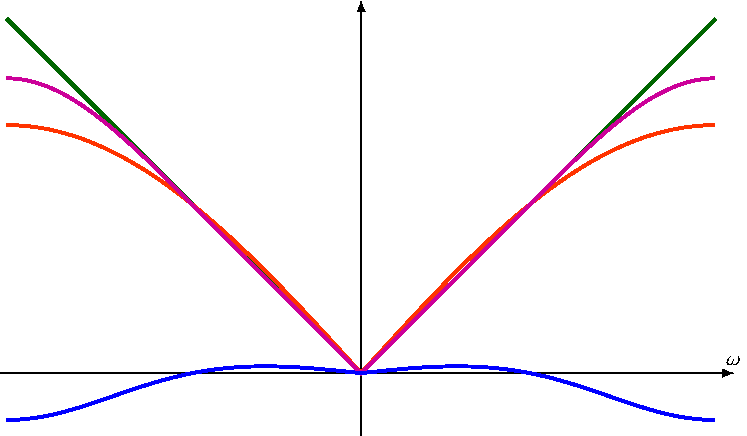
\includegraphics{papers/interdiff/experiment.pdf}
\caption{Fourier-Transformierte der Koeffizientenfolge für die Ableitung 
basierend auf dem Interpolationspolynom.
\label{interdiff:spektrum}}
\end{figure}
Die Fourier-Transformation der Ableitung einer Funktion ist
\[
\mathcal{F}
\frac{df}{dx}
=
i\omega\mathcal{F}f.
\]
Dies gibt uns eine Möglichkeit, die Qualität der Ableitungsmethoden
von Abschnitt~\ref{section:interdiff:ableitung} zu messen.
Diese Berechnungsmethode ist eine Faltung mit der Folge der
Ableitungskoeffizienten.
Im Frequenzbereich wird daraus eine Multiplikation mit der
Fourier-Transformierten.
Der absolute Betrag der diskrete Fourier-Transformierten
der Ableitungskoeffizienten müsste also eine Betragsfunktion ergeben.

Die Resultate der Rechnung sind in Abbildung~\ref{interdiff:spektrum}
dargestellt.
Die Betragsfunktion ist grün dargestellt,
der gewöhnliche Differenzenquotient in hellrot.
Die pinke Kurve zeigt das Ableitungsverfahren, welches acht
Stützstellen verwendet.
Ganz offensichtlich wird dadurch das ideale Spektrum der
Ableitung besser approximiert.
Man kann allerdings auch erkennen, dass das Verfahren höhrer Ordnung
die hohen Frequenzen verstärkt, es ist also anfälliger auf Rauschen.





\printbibliography[heading=subbibliography]
\end{refsection}
